\documentclass[../main.tex]{subfiles}
\graphicspath{{\subfix{../images/}}}
\begin{document}
	
	\chapter{Methods}
		\section{Developing the characterization procedure}
		One of the aims of this project is to develop an experimental procedure that enables us to characterize the camera that may be flown on the STEP mission. This characterization is crucial in order to test the validity of the scientific goals for the mission. Such a procedure should be exactly reproducible, such that we can ensure its correctness.
	
		\subsection{Preliminary thoughts and considerations}
		\subsubsection{Acquiring data and reducing noise}
		Characterization of a CCD chip involves acquiring image frames in a variety of way to study several effects. We study effects by acquiring frames while varying a parameter like temperature (thermal noise) or exposure time (linearity). For each value of this varied parameter, say temperature for thermal noise (dark current), we wish to associate a functional value, here electrons per second in the example at hand. This is done by considering the frame taken at that value of the variable (temperature), and computing the mean value of the experimental metric (dark current, electrons per second) across all pixels in the image. For any measurement, we should take steps to reduce the noise in the image. Dark current can be reduced by cooling the chip before acquiring data frames. Readout noise is \textbf{gaussian} and the noise in the distribution is reduced by a factor of $1/\sqrt{N}$ for $N$ measurements. Hence, for each datapoint, before computing the desired variable, like dark currrent for a specific temperature, we should, at that temperature, acquire $N$ frames, and construct a mean image from these $N$ frames. Typically $N$ is chosen to be as large as is practically feasible. The value of the experimental metric is then computed from that average frame. 
	
		\subsubsection{Background noise and Dark current}
		In order to find a good starting point for the development of the testing procedure, a preliminary investigation of the noise levels of the chip was carried out. This was done at a desktop in an office, using a very primitive experimental setup. This preliminary test confirms that dark current is strongly dependent on temperature. See figure \ref{fig:dcprelim}. Since the camera cooler is only able to cool to a temperature gradient of $\Delta T = 30 ^\circ $C, the temperature $T = -10 ^\circ$ C was chosen since we cannot be sure that we can feasibly stay at a lower temperature, if room temperature varies. This should ensure that we can minimize dark current and read-out noise.
		\begin{figure}
			\centering
			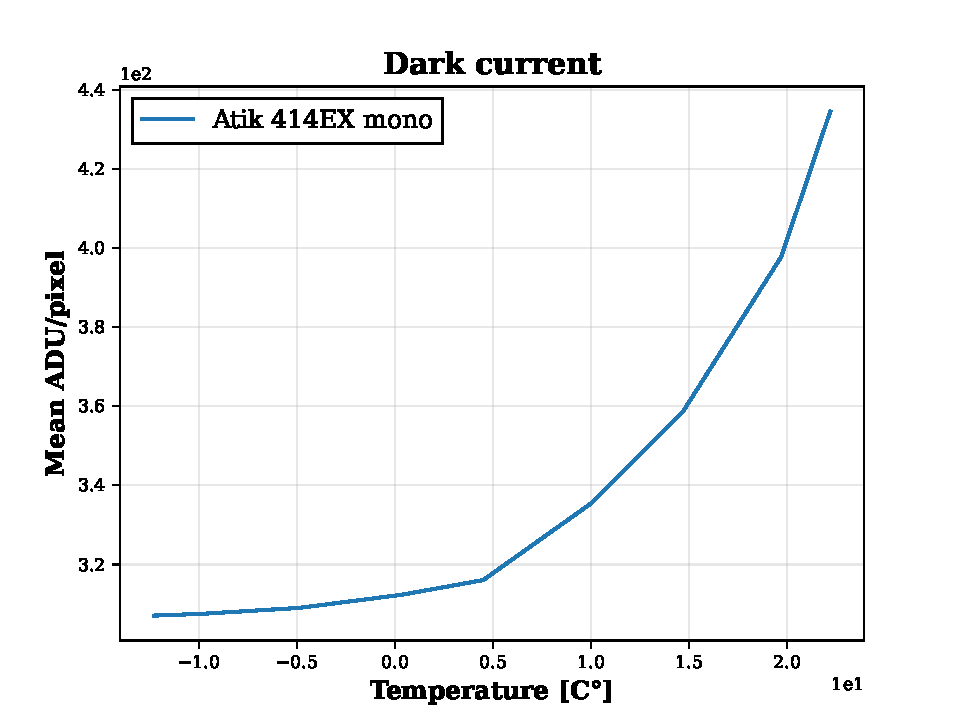
\includegraphics[width=0.6\textwidth]{dark_current_versus_temperature.pdf}
			\caption{Preliminary dark current measurement, performed at the office in sub-optimal settings, to get a first glimpse of the behaviour of this variable.}
			\label{fig:dcprelim}
		\end{figure}
		
		\subsubsection{Master bias and flat field frames}
		$300$ images are acquired at exposure times of $0.001$ seconds. From these a \textbf{master bias} frame can be constructed. This frame should be subtracted from all other data points, and represents a bias voltage applied to the chip, in order to avoid negative values in the ADC. This effect is also studied as a function of temperature via the readout noise (RON) effect. 
		In addition flat field frames ($300$ frames) are acquired as well, and meaned over, subtracting the master bias. All of these frames are acquired at the $T= -10^\circ$ temperature setpoint chosen above.
		
		\subsubsection{The initial experimental setup}
		The initial setup used with this camera, to carry out the testing and characterization procedure, can be seen in figure \ref{fig:setup}. 
		
		\begin{figure}
			\centering
			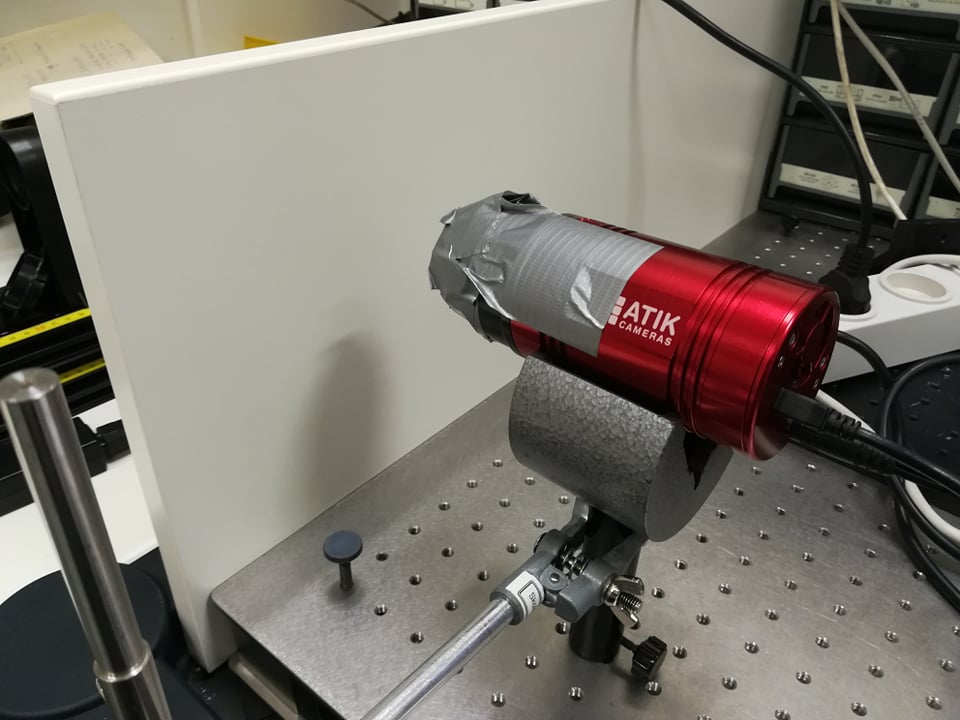
\includegraphics[width=0.6\textwidth]{setup.jpg}
			\caption{Initial experimental setup, which was used both for the light and dark exposures.}
			\label{fig:setup}
		\end{figure}
		
		The setup consists of the aforementioned camera in question, which is resting on a stand, pointed into a white lacquered wooden screen. The camera is connected via USB2 to the lab-computer, and is additionally connected to a power supply. Since the setup for dark frames simply require a sufficiently dark room, an in house dark-room is used.
		For all light exposures the ambient room lighting was used, and the camera (with a pinhole mounted with tape, constructed from heavy black cardboard) was pointed into the screen. 
		For all dark frames, the same configuration was used, but with no ambient light, and computer screens turned off.
		
		\subsubsection{Exposure times for linearity}
		The linearity measurement consists of acquiring exposures of the white screen, as a function of exposure time, in order to study the linearity of the response in measured photons by the detector. Hence we should first determine which exposure time interval to use. At first a 100s exposure acquisition was carried out, in which considerable saturation was observed. From this it was concluded that an exposure time of 100 seconds was a good 'datapoint' to use for the last acquisition. The choice of exposure times relies on trial and error, to decide what range of exposure times we should use, at a given light source intensity. At first frames at exposures between $0.001s$ and $110s$ in $5s$ intervals was acquired. It was found that the light source stability varies significantly, resulting in greater uncertainty in short exposure measurements, and hence it was chosen to omit $0$ seconds, and instead acquire frames in the interval $1s$ to $10s$ in 1 second intervals, in addition to the data sequence described just above. 
		
		\subsubsection{Noise as a function of temperature}
		Readout noise and dark current are expected to be temperature dependent, and hence, in the entire cooling range of the camera, it is interesting to acquire images of dark frames in order to study the behaviour of these physical effects. Exposure times are chosen such that the minimal exposure time is chosen for the readout noise images, since no photon should have been detected, and since dark current is time dependent, and hence should be negligible in this regime. For dark current frames, it is crucial to pick an exposure time such that the dark current contribution is greater (by a considerable amount, higher orders of magnitude) than the readout noise contribution. Dark current follows a \textbf{poissonian} distribution, and to recover this underlying distribution we should pick long exposure times. Since this require \textbf{very} long times of exposure, it is more practical to pick an exposure time of $10s$, and then mean over $100$ acquired images at this temperature, to reduce the noise contribution, since readout noise should be gaussian with a zero-centered mean value. 
		
		\subsubsection{Hot pixel treatment}
		It is crucial to treat hot pixels. One way to do this, is to realize that hot pixels, are those pixels in which dark current does not show a linear temporal behaviour. Acquiring a \textit{very} long exposure, and a medium long (considerably shorter than the former) exposure, we can study the dark current in each pixel, and determine if there is a linear relationship between the two frames. This is done by scatterplotting the pixels, and findin (qualitatively) the range within which the data points seem to follow a linear relationship. The remainder are considered hot in this sense, and from this information a mask can be constructed. These pixels can then be omitted in mean values used in the other analyses.
		
		\subsubsection{Testing of ground assumptions}
		In our experimental setup, assumptions have been made that need to be tested. The two most important ones, which enable the testing of linearity are that 
		\begin{itemize}
			\item The camera has a well-calibrated zero point temporally. That is to say that a 10 second exposure is actually physically the frame resulting from light being able to enter the chip for exactly 10 seconds.
			\item The ambient light source in the room is stable during exposure, so we can accurately compare ADU intensities between different frames.
		\end{itemize}
		The latter assumption can be tested by analyzing the many exposures taken during the linearity sequence, by plotting the percentage deviation, from the mean ADU (mean across all 100 exposures at a given exposure time) as a function of exposure number.
		
		\subsection{Stability of the lightsource}
		That the light source used for the light exposures, is stable is one of two ground assumptions that went into the experimental setup. This assumption should be tested, since we can generally not expect a flourescent light bulb, connected to the main relay, to be stable to a high precision. At first, this was tested by utilizing the wealth of data acquired during the linearity measurement sequence. At each exposure interval, $100$ consecutive frames were acquired. This enables us to plot the intensity as a function of time. This was done by considering the series of images, say the series of images taken at a $30s$ exposure time. From this series a mean image was constructed. The mean ADU/pixel in this image is our reference value. The percentage deviation in the mean ADU/pixel, in each of the individual frames, was then plotted as a function of time (repeat numbers, properly speaking). This way it was possible to qualitatively judge the stability of the lightsource as a function of time. Such a plot can be seen in figure \ref{fig:lightsourcestability}. It is clear that, save for a few of the exposure times, the lighting is only stable to a few percentage points deviation. This gives us a first estimate of the instability, indicating that we should attempt to correct for this source of systematic error. 
		
		\begin{figure}
			\centering			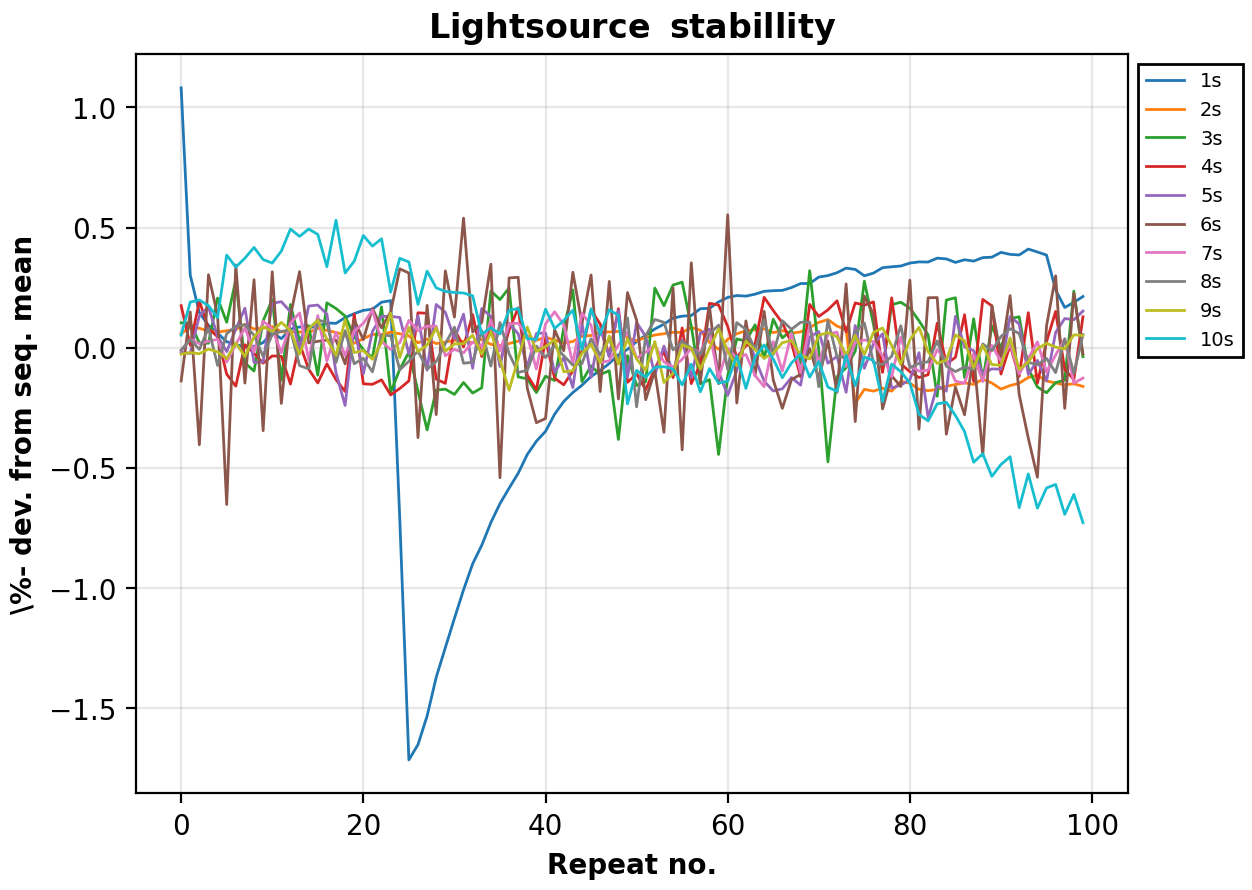
\includegraphics[width=0.8\textwidth]{lightsource.png}
			\caption{A plot of the temporal dependence in the lightsource intensity (flux) across each of the different exposure times. Numbering is ordered according to the preliminary series of exposure times as described in the text.}
			\label{fig:lightsourcestability}
		\end{figure}
		
		These deviations from perfect stability can not be used as a correction, since this does not include the correlation of instability between exposure times. Instead it is proposed that a reference exposure is utilized. Within a given repeat sequence, one may use a reference of $10s$ exposure by alternating between the chosen reference exposure, and the actual desired exposure. Such an exposure series is akin to $[10s, 1s, 10s, 1s, 10s, \dots 10s, 2s, 10s, 2s,\dots]$ covering the entire range. For each actual frame we then have a 10 second exposure just before and right after. For the test procedure camera, the software designed for the camera, only enables the user to set up a sequence of 10 data points to be acquired automatically, but allows for that sequence to be repeat. hence it was most practical for the analysis to acquire data in the series $[10s, 1s, 10s, 2s, 10s, 3s, 10s, \dots 10s, 9s, 10s]$, repeat that N times ($N=10$ was chosen due to time constraints), and then repeat until the desired exposure time range has been covered. The two reference measurements to use in correction of a given frame will then be the two taken at adjacent times. 
		
		The flux of the light source at the time of our desired frame then lies somewhere in between, assuming no wild fluctuations or drifts, and a linear change in the time in between acquisition of the two reference frames. These assumptions of local monotonicity of the light source flux are justified by considering figure \ref{fig:lightsourcestability}. Let $\bm F(x[s]) = \text{mean}\left(\text{Image}([s])\right)$ be interpreted as the mean flux in an image of exposure time $s$ in seconds, that is, the mean ADU value of an arbitrary image of exposure time $s$. Hence we may correct for the instability, using a 10 second reference exposure, for a given frame via the computation
		\begin{equation}\label{eq:fluxcorrect_notimecal}
			\bm F(x [s])_\text{corrected} = \frac{\bm F(x [s])}{\frac12\left[\bm F(10s)_\text{before}+\bm F(10s)_\text{after}\right]} * 10
		\end{equation}
		Where the last factor of 10 is to account for the relation between the 10 second and 1 second exposure times, in the ideal case where there is no time offset.
		
		\subsection{Time calibration}
		Another assumption is one that pertains to the camera itself, the time calibration of the measurements. A series of measurements was constructed in order to study whether or not the zero point of the camera imaging was actually at $0s$ and to what precision. A preliminary estimate can be studied by acquiring eight frames, by noting that, under the assumption that our detector is linear, it should be true that for a given frame $\text{Image}(\text{Exposure time})$, we must expect for a perfect time calibration that 
		
		\begin{equation}
			\frac{\text{Image}(21s) - \text{Image}(1s)}{\text{Image}(11s) - \text{Image}(1s)} = \frac{\text{Image}(10s) - \text{Bias}}{\text{Image}(20s) - \text{Bias}}
		\end{equation}
		Or that 
		\begin{equation}
			\frac{\textbf{mean}(\text{Image}(21s) - \text{Image}(1s))}{\textbf{mean}(\text{Image}(11s) - \text{Image}(1s))} - \frac{\textbf{mean}(\text{Image}(10s) - \text{Bias})}{\textbf{mean}(\text{Image}(20s) - \text{Bias})} = 0
		\end{equation}
		where \textbf{mean}$()$ refers to the mean ADU/pixel within an image. The result of this, for the test procedure camera, being $0.0063$ indicates a time offset which must be determined properly, and applied as a correction. The test procedure camera does not have a shutter, and the data sheet \cite{atik414specs}, specifies a $1/15 s$ readout time. Hence an exposure time of $1s$ should correctly be interpreted as an exposure time of $1s + \Delta t$, where $\Delta t$ should be deduced experimentally. Via a seperate linearity measurement series with greater precision (more datapoints) in the uncertain interval of $1s - 10s$ in which this readout time would actually be able to significantly impact exposure times, we can get a first estimate of $\Delta t$ by fitting a linear function to the data points, and determining the roots of polynomium. If there is a time offset, the line will intersect the first axis at a point different from the origin. The intersection point on the first axis should be subtracted. For a negative value of the intersect point on the first axis, a subtraction physically corresponds to a longer exposure time. We should then correct for this time offset by adjusting the equation \ref{eq:fluxcorrect_notimecal}, and achieving a the same time the true measure of unlinearity, $\delta$ as
		\begin{equation}\label{eq:fluxcorrect_timecal}
		\delta = \left( \frac{\bm F(x [s])}{\frac12\left[\bm F(10s)_\text{before}+\bm F(10s)_\text{after}\right]}\frac{10s + \Delta t}{x [s] + \Delta t} - 1 \right) * 100\%
		\end{equation}
		
		\subsection{Shutter test}
		
		
		
		\section{Measurement plan}
		
		\subsection{Linearity}
		For each exposure time in the series 
		$[1, 2, \dots 9, 10, 15, 20, \dots 100, 105, 110]$, all in units of seconds, with a $10$ second reference frame as described above, was acquired, with $N = 10$ repeats which are then meaned over in order to reduce readout noise levels. The unlinearity is computed according to equation \ref{eq:fluxcorrect_timecal} for each exposure time after meaning across $N$ frames. This produces a plot like figure \ref{fig:linearity}
		
		\begin{figure}
			\centering			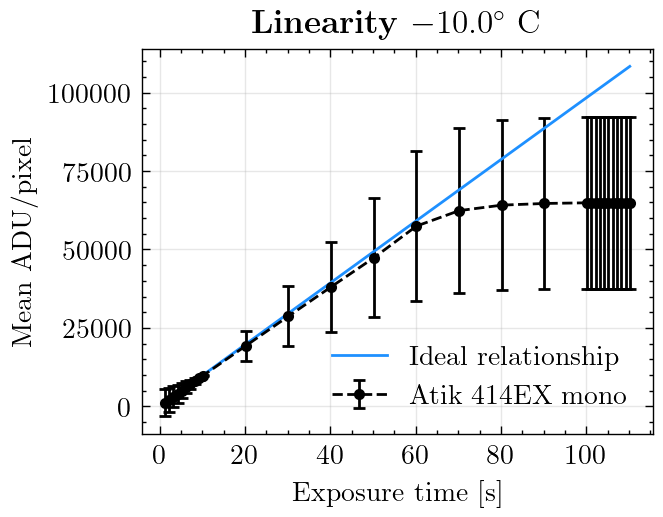
\includegraphics[width=0.65\textwidth]{linearity.png}
			\caption{A plot of the percentage deviation from ideal linearity, computed according to equation  \ref{eq:fluxcorrect_timecal} for each exposure time after meaning across $N$ frames. }
			\label{fig:linearity}
		\end{figure}
		
		\subsection{Temperature dependence of noise}\label{sec:rondc}
		For each temperature in the series $[-10, -8, -6, -4, -2, 0, 2, 4, 6, 8, 10, 12, 14, 16, 18, 20]$ all in $^\circ $C, 100 bias frames at $0.001$s, and 100 dark frames at $10.0s$ for each temperature was acquired. The former was used to compute the readout noise as a function of temperature. Each temperature sequence was considered. As an example consider the one for $-8^\circ$C. For this series, each repeat image was considered in turn, and the mean ADU/pixel was computed and subtracted form every pixel in the image. This resultant image was a stochastic distribution around zero. We expect this to be a gaussian distribution. By multiplying with the camera gain factor in each pixel, we can interpret the width of this distribution as the readout noise, in units of electrons. The standard deviation was computed from the flattened array of pixels to obtain the width. This yielded, for a temperature sequence, $100$ standard deviations. From this a RMS value was computed. These values can then be plotted as a function of temperature.
		
		The dark current data was treated in much the same way. For each temperature sequence, a mean image was constructed in order to reduce the readout noise contamination in the image. This picture was then multiplied with the camera gain factor, and divided by the exposure time according to equation \ref{darkcurrenteq}, and from this the mean ADU/pixel was computed. This is plotted as a function of temperature. 
		
		The result of these two anlysis may be seen plotted in figure \ref{fig:noise}	
		
		\begin{figure}
			\centering			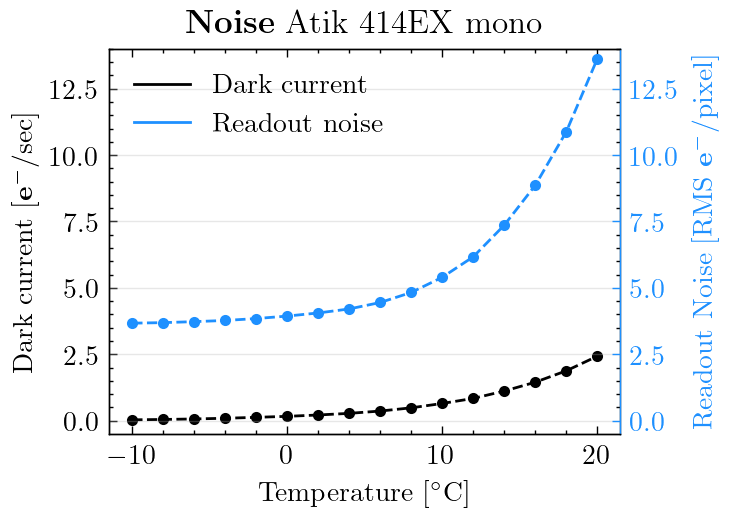
\includegraphics[width=0.65\textwidth]{noise_versus_temperature.png}
			\caption{Dark current and readout noise as a function of temperature. The datapoints have been constructed by acquiring 100 dark frames at exposure times $0.001$ s for readout noise, and $10$s for dark current, at each temperature. Readout noise is computed according to section \ref{sec:rondc}, and dark current according to equation \ref{darkcurrenteq}. }
			\label{fig:noise}
		\end{figure}
	
\end{document}